\section{$NO_x$ Sensor Cross-sensitivity}
Commercial $NO_x$ sensors are cross-sensitive to tailpipe ammonia. The resulting error is modelled as a function of
ammonia concentration and a temperature-dependent cross-sensitivity factor $\chi(T)$. This introduces a non-negative
directional error $\lr{\varepsilon_\chi}$ into the tailpipe $NO_x$ measurement $\con{NO_x}^{out}_{\chi}$
(Figure~\ref{fig::cross_sen_ref1}).
\begin{align}
        \varepsilon_\chi= \chi\lr{T(k)} \times \con{NH_3}^{out}\geq 0
\end{align}
%===
\begin{figure}[!ht]
        \centering
        \includegraphics[width=\figWidth]{./figs/2-data/cross_aged_hftp.png}
        \caption{$NO_x$ sensor cross-sensitivity to tailpipe ammonia}
        \label{fig::cross_sen_ref1}
\end{figure}
The FTIR sensor also has a bias that is directional.

\subsection{$NO_x$ sensor cross-sensitivity Estimation}
The sensor cross-sensitivity $\chi$ can be estimated using the FTIR (Fourier transform infrared) sensor data ($x_1$)
along with the actual sensor measurement data ($y_1$) and the ammonia concentration measurement ($x_2$). We have,
\begin{align*}
    y_1 &= x_1 + \chi x_2
\end{align*}
Note that the FTIR sensor has bias (and drift) that have to be corrected for. Let $x_b$ be the biased sensor data and
$b$ be the bias.
\begin{align*}
    x_b &= x + b(t)
\end{align*}
\subsubsection{Bias correction}
The value of $b$ is assumed to linearly change with time: this assumption captures the linear drift in the sensor as
well.
\begin{align*}
    b(t) &= b_1 t + b_0
\end{align*}
$b_1$ and $b_0$ are estimated using the bias at the starting segment and the tail end of the data can fit the change
linearly with time.
\begin{figure}[!ht]
    \begin{minipage}{0.49\textwidth}
        \begin{figure}[H]
            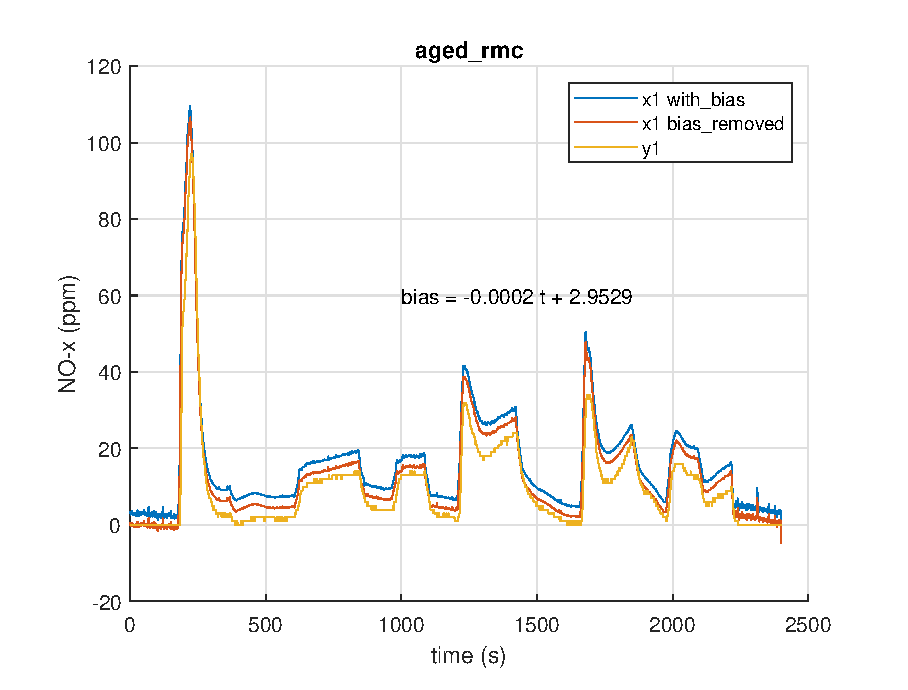
\includegraphics[width=\textwidth]{./figs/2-data/chi_est/aged_rmc_NOx_bias.eps}
        \end{figure}
    \end{minipage}
    \begin{minipage}{0.49\textwidth}
        \begin{figure}[H]
            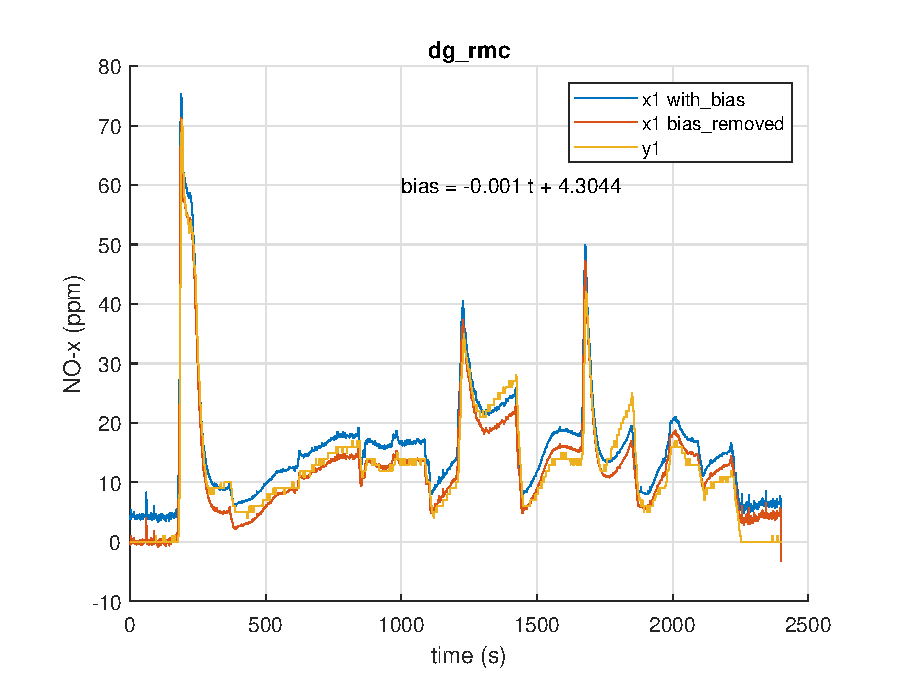
\includegraphics[width=\textwidth]{./figs/2-data/chi_est/dg_rmc_NOx_bias.eps}
        \end{figure}
    \end{minipage}
        \caption{Sensor bias correction for RMC cycles}
        \label{fig::bias_corr}
\end{figure}
The results depicted in Figure~\ref{fig::bias_corr} indicate that the coefficient of \( t \), \( b_1 \) (drift), is
considerably smaller in comparison to the bias \( b_0 \), suggesting it can be disregarded.

\subsubsection{Effect of $NH_3$ sensor bias and minimum threshold for cross-sensitivity}
The ammonia sensor used for ammonia measurement also has bias and there is a threshold on ammonia for which the $NO_x$
sensor becomes cross-sensitive to ammonia. Thus the expression for cross-sensitivity becomes:
\begin{align*}
    y_1 &= \lr{x_1 - b_0} + \chi (x_2 - b_{th})\\
\end{align*}

\subsubsection{Least-squares estimation assuming temperature independence}
The temperature changes in the RMC cycle do not affect the cross-sensitivity factor significantly. Thus, it can be treated as
a constant with respect to temperature fluctuations in that range. We have,
\begin{align*}
    \underbrace{y_1 - x_1}_{\pmb y} &= \underbrace{\bm{x_2 & -1}}_{\pmb \phi^T} \underbrace{\bm{ \chi \\ \underbrace{\chi b_{th} + b_0}_{=b}}}_{ \pmb \theta}\\
\end{align*}
Using the above model, the least-squares estimation of $\chi$ and $b$ is performed for RMC cycles. The results are shown
in Figure~\ref{fig::chi_est} and the error in estimation is shown in Figure~\ref{fig::chi_error}.
\begin{figure}[!ht]
    \begin{minipage}{0.49\textwidth}
        \begin{figure}[H]
            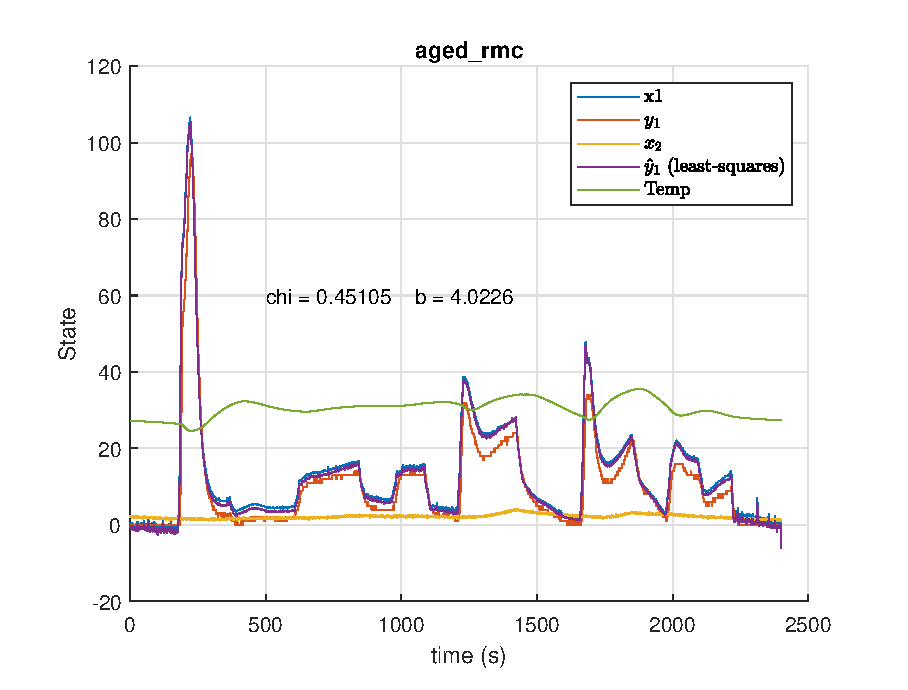
\includegraphics[width=\textwidth]{./figs/2-data/chi_est/aged_rmc_chi.eps}
        \end{figure}
    \end{minipage}
    \begin{minipage}{0.49\textwidth}
        \begin{figure}[H]
            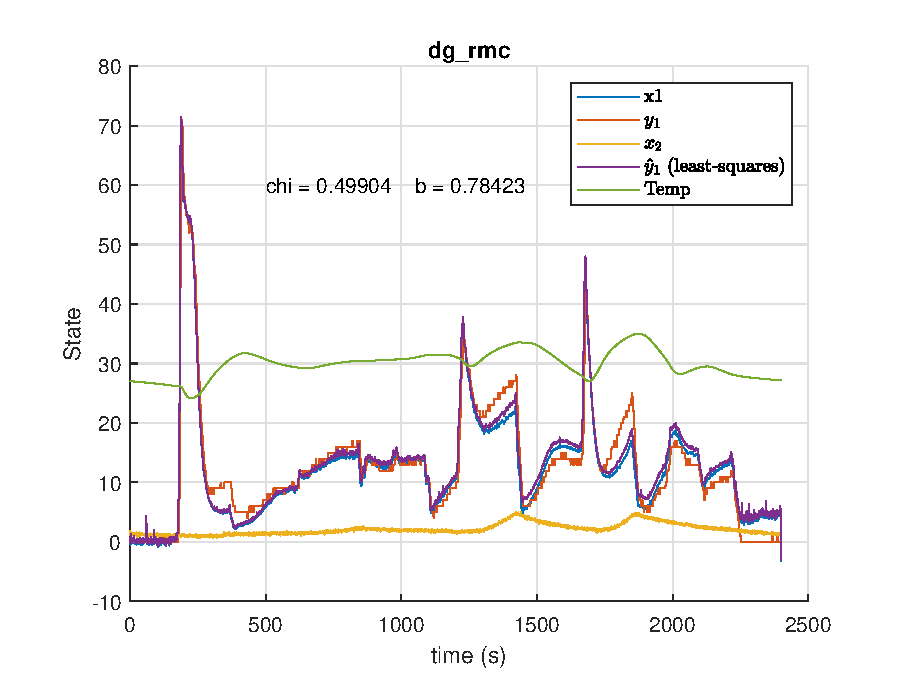
\includegraphics[width=\textwidth]{./figs/2-data/chi_est/dg_rmc_chi.eps}
        \end{figure}
    \end{minipage}
        \caption{$\chi$ estimation for RMC cycles}
        \label{fig::chi_est}
\end{figure}
\begin{figure}[!ht]
    \centering
    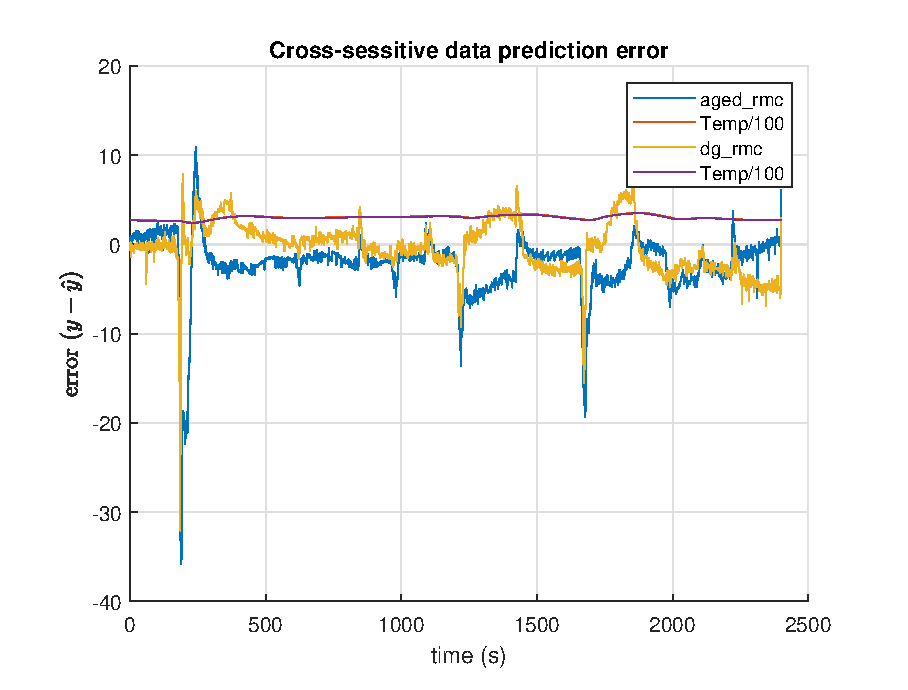
\includegraphics[width = 0.5 \textwidth]{./figs/2-data/chi_est/chi_error.eps}
    \caption{Error in $\chi$ estimation}
    \label{fig::chi_error}
\end{figure}
The error can be reduced by introducing the effects of temperature into $\chi$.

\subsubsection{Least-squares estimation with $\chi$ as a temperature function}
For simplicity, $\chi$ is assumed to be a linear function of temperature.
\begin{align*}
    \chi(T) &= a T - b_T
\end{align*}
Assuming the sensor-bias is not time-varying ($\because$ $b_1$ is small). The sensor bias, cross-sensitivity threshold
and temperature dependence can be combined into:
\begin{align*}
    y_1 &=  \lr{x_1 - b_0} + \lr{aT - b_{T}} \lr{x_2 - b_{th}}\\
    \lr{y_1 - x_1} &= a T x_2 - a b_{th} T - b_{T} x_2 + (b_T b_{th} - b_0)\\
    \underbrace{y_1 - x_1}_{\pmb y} &= \underbrace{\bm{T x_2 & -T & -x_2 & 1}}_{\pmb \phi^T} \underbrace{\bm{a \\ a b_{th} \\ b_T \\ b_T b_{th} - b_0}}_{\pmb \theta}\\
\end{align*}
The least-squares estimation of the parameters is performed using the above model and the results are shown in Figure~\ref{fig::chi_est_T} and the error in estimation is shown in Figure~\ref{fig::chi_error_comp}.
\begin{figure}[!ht]
    \begin{minipage}{0.49\textwidth}
        \begin{figure}[H]
            \includegraphics[width=\textwidth]{./figs/2-data/chi_est/aged_rmc_chiT.eps}
        \end{figure}
    \end{minipage}
    \begin{minipage}{0.49\textwidth}
        \begin{figure}[H]
            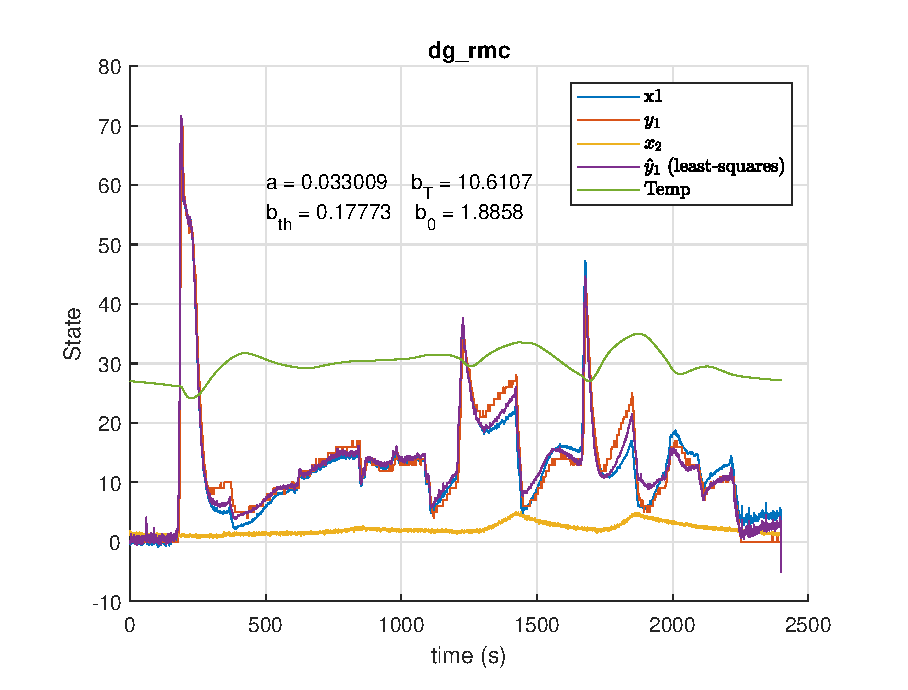
\includegraphics[width=\textwidth]{./figs/2-data/chi_est/dg_rmc_chiT.eps}
        \end{figure}
    \end{minipage}
        \caption{$\chi$ estimation for RMC cycles}
        \label{fig::chi_est_T}
\end{figure}
\begin{figure}[!ht]
    \begin{minipage}{0.49\textwidth}
        \begin{figure}[H]
            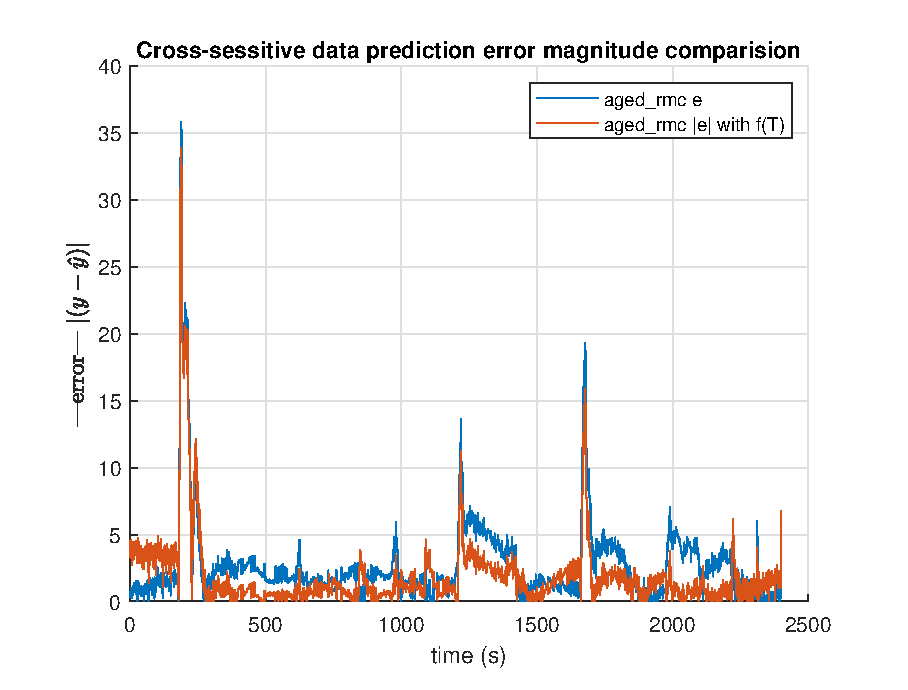
\includegraphics[width=\textwidth]{./figs/2-data/chi_est/aged_error_comp.eps}
        \end{figure}
    \end{minipage}
    \begin{minipage}{0.49\textwidth}
        \begin{figure}[H]
            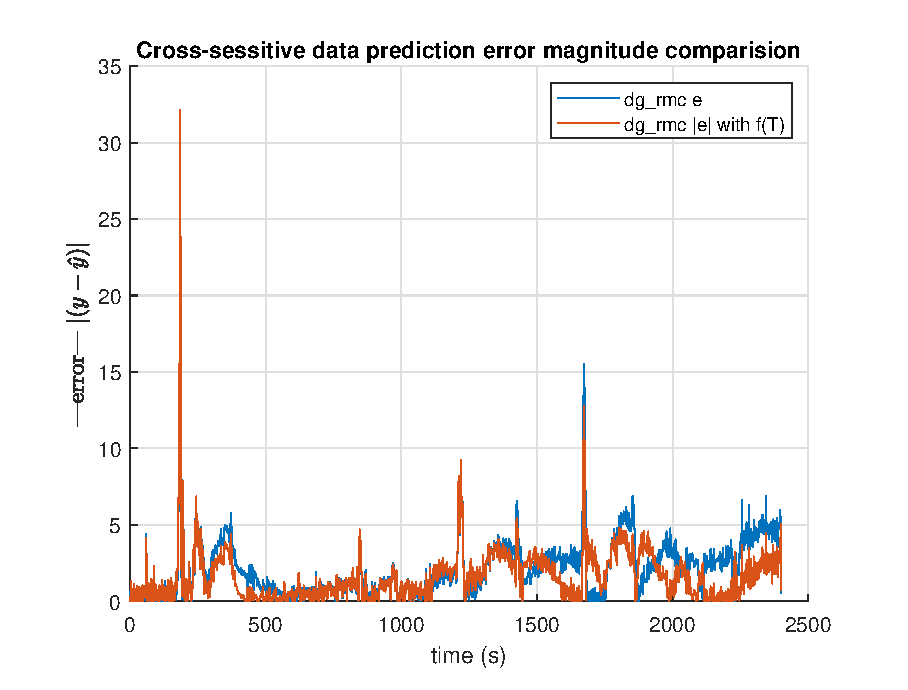
\includegraphics[width=\textwidth]{./figs/2-data/chi_est/dg_error_comp.eps}
        \end{figure}
    \end{minipage}
        \caption{Effect of temperature on prediction errors for $\chi$ estimation in RMC cycles}
        \label{fig::chi_error_comp}
\end{figure}
Introducing temperature clearly decreases the prediction error (Figure~\ref{fig::chi_error_comp}) in the model. However,
the reduction in error, while noticeable, is not significant when compared to the temperature-independent model
(Figure~\ref{fig::chi_error}), whose error remains within acceptable limits. Moreover, tailpipe ammonia measurements are
required for estimation of the cross-sensitivity error. Hence, for the current work, the cross-sensitivity effect is
treated as an unknown bounded disturbance.
